\documentclass[11pt, aspectratio=169]{beamer}
\usetheme{Madrid}
\usepackage[T1]{fontenc}
\usepackage{graphicx}
\usepackage{booktabs}
\usepackage{tabularx}
\usepackage{tikz}
\usetikzlibrary{arrows.meta, positioning, calc, decorations.pathreplacing}

% ---------- Palet warna bertema kebangsaan ----------
\definecolor{merahps}{RGB}{193,39,45}
\definecolor{emasps}{RGB}{184,134,11}
\definecolor{birutuaps}{RGB}{17,45,78}

\setbeamercolor{structure}{fg=merahps}
\setbeamercolor{title}{fg=birutuaps}
\setbeamercolor{palette primary}{fg=white,bg=merahps}
\setbeamercolor{palette secondary}{fg=white,bg=birutuaps}
\setbeamercolor{palette tertiary}{fg=white,bg=birutuaps}
\setbeamercolor{section in toc}{fg=birutuaps}
\setbeamercolor{frametitle}{fg=white,bg=birutuaps}
\setbeamerfont{frametitle}{series=\bfseries}
\setbeamertemplate{navigation symbols}{}

\let\olditem\item
\renewcommand{\item}{\olditem\vspace{4pt}}

\title[Penerapan \& Dinamika PPKN]{Penerapan Nilai Pancasila dan Dinamika UUD NRI Tahun 1945}
\author[Kelompok 2]{
    Aliif$^1$ \and
    Avis$^2$ \and
    Azzahra$^3$ \and
    Regita$^4$ \and
    Wisam$^5$
}
\institute[SMK]{SMK Plus Pratama Adi}
\date{\today}

\begin{document}

% =========================================================
\begin{frame}
    \titlepage
    \vspace{-0.4cm}
    \begin{center}
        {\footnotesize\itshape ``Di atas dasar Pancasila, kita mendirikan negara Indonesia yang kekal dan abadi.'' --- Ir.Soekarno}
    \end{center}
\end{frame}

% =========================================================
\begin{frame}{Daftar Isi}
    \tableofcontents
\end{frame}

% =========================================================
\section{Penerapan Nilai-Nilai Pancasila}

\begin{frame}{Asal Mula dan Kedudukan Pancasila}{A. Asal Mula dan Kedudukan Pancasila}
    \begin{itemize}
        \item Pancasila adalah \textbf{pandangan hidup bangsa}: nilai-nilainya telah hidup dalam
        masyarakat Indonesia jauh sebelum merdeka.
        \item Semboyan \textbf{Bhinneka Tunggal Ika} diambil dari Kitab \textit{Sutasoma} karya
        Mpu Tantular pada masa Kerajaan Majapahit.
        \item Menurut \textbf{Kaelan (2020)}, secara kausalitas asal mula Pancasila terbagi menjadi
        empat unsur (lihat diagram pada slide berikutnya).
        \item Nilai-nilai Pancasila hidup dalam tiga tataran: nilai dasar, nilai instrumental, dan
        nilai praksis.
    \end{itemize}
\end{frame}

% ---------------------------------------------------------
\begin{frame}{Empat Kausa Asal Mula Pancasila}
    \begin{center}
    \resizebox{0.88\linewidth}{!}{%
    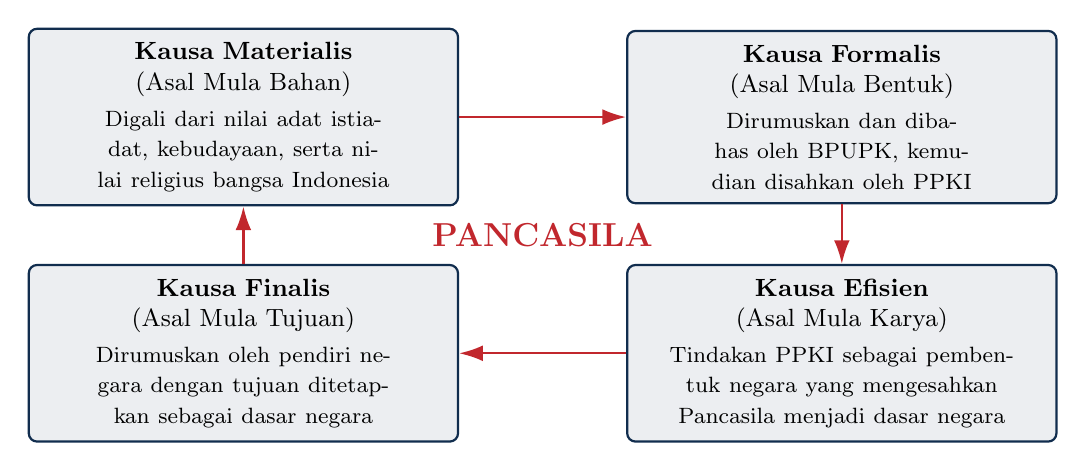
\begin{tikzpicture}[
        every node/.style={font=\small},
        box/.style={rectangle, rounded corners=3pt, draw=birutuaps, thick,
                    fill=birutuaps!8, text width=5.1cm, minimum height=2.0cm,
                    align=center, inner sep=5pt},
        arr/.style={-{Latex[length=3mm,width=2mm]}, thick, merahps}
    ]
        \node[box] (mat)  at (0,2.9)   {\textbf{Kausa Materialis}\\(Asal Mula Bahan)\\[2pt]
            \footnotesize Digali dari nilai adat istiadat, kebudayaan, serta nilai religius
            bangsa Indonesia};
        \node[box] (form) at (7.6,2.9) {\textbf{Kausa Formalis}\\(Asal Mula Bentuk)\\[2pt]
            \footnotesize Dirumuskan dan dibahas oleh BPUPK, kemudian disahkan oleh PPKI};
        \node[box] (efi)  at (7.6,-0.1){\textbf{Kausa Efisien}\\(Asal Mula Karya)\\[2pt]
            \footnotesize Tindakan PPKI sebagai pembentuk negara yang mengesahkan Pancasila
            menjadi dasar negara};
        \node[box] (fin)  at (0,-0.1)  {\textbf{Kausa Finalis}\\(Asal Mula Tujuan)\\[2pt]
            \footnotesize Dirumuskan oleh pendiri negara dengan tujuan ditetapkan sebagai
            dasar negara};
        \draw[arr] (mat.east)  -- (form.west);
        \draw[arr] (form.south)-- (efi.north);
        \draw[arr] (efi.west)  -- (fin.east);
        \draw[arr] (fin.north) -- (mat.south);
        \node[merahps, font=\bfseries\large] at (3.8,1.4) {PANCASILA};
    \end{tikzpicture}}
    \end{center}
    \vspace{1mm}
    {\scriptsize\centering Keempatnya membentuk satu kesatuan sebab-akibat yang saling menguatkan kedudukan Pancasila sebagai dasar negara.\par}
\end{frame}

% ---------------------------------------------------------
\begin{frame}{Tiga Tataran Nilai dalam Ideologi Pancasila}
    \begin{center}
    \resizebox{0.95\linewidth}{!}{%
    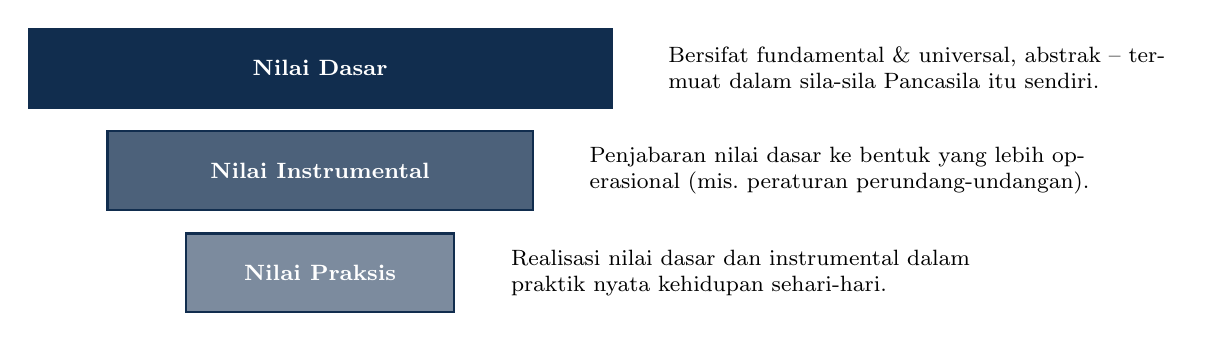
\begin{tikzpicture}[font=\small,
        bar/.style={draw=birutuaps, thick, minimum height=1.0cm, align=center,
                    font=\bfseries\footnotesize, text=white}
    ]
        \node[bar, fill=birutuaps,     minimum width=7.4cm] (dasar)   at (0,0)    {Nilai Dasar};
        \node[bar, fill=birutuaps!75,  minimum width=5.4cm] (instr)   at (0,-1.3) {Nilai Instrumental};
        \node[bar, fill=birutuaps!55,  minimum width=3.4cm] (praksis) at (0,-2.6) {Nilai Praksis};

        \node[align=left, text width=6.4cm, font=\footnotesize, anchor=west] at (4.3,0)
            {Bersifat fundamental \& universal, abstrak -- termuat dalam sila-sila Pancasila itu sendiri.};
        \node[align=left, text width=6.4cm, font=\footnotesize, anchor=west] at (3.3,-1.3)
            {Penjabaran nilai dasar ke bentuk yang lebih operasional (mis.\ peraturan perundang-undangan).};
        \node[align=left, text width=6.4cm, font=\footnotesize, anchor=west] at (2.3,-2.6)
            {Realisasi nilai dasar dan instrumental dalam praktik nyata kehidupan sehari-hari.};
    \end{tikzpicture}}
    \end{center}
\end{frame}

% ---------------------------------------------------------
\begin{frame}{Pembudayaan Pancasila: Investasi Karakter}{B. Pembudayaan Pancasila dan Investasi Karakter}
    \begin{itemize}
        \item Pembudayaan Pancasila bertujuan mewujudkan tujuan negara dengan mengedepankan
        potensi kecerdasan (\textit{civic intelligence}).
        \item \textbf{Ir. Sukarno} menggagas \textbf{Revolusi Mental} (\textit{Nation and Character
        Building}) untuk membangun mentalitas bangsa secara menyeluruh.
        \item Dalam pendidikan karakter, ajaran keteladanan \textbf{Ki Hajar Dewantara} sangat
        penting untuk diterapkan melalui tiga posisi kepemimpinan (lihat slide berikutnya).
    \end{itemize}
\end{frame}

\begin{frame}{Trilogi Kepemimpinan Ki Hajar Dewantara}
    \begin{center}
    \resizebox{0.95\linewidth}{!}{%
    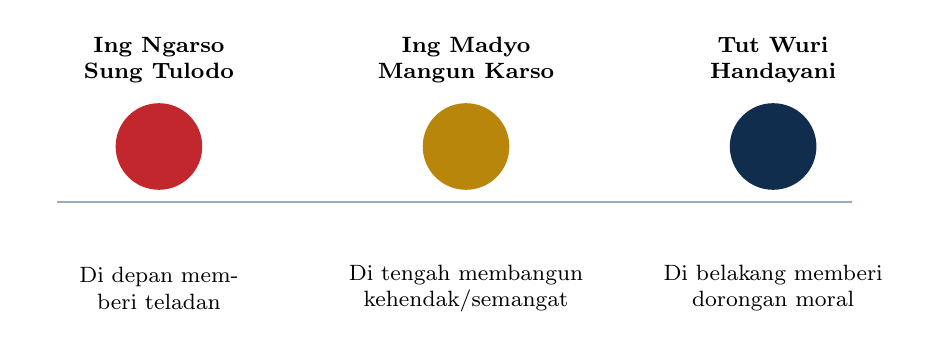
\begin{tikzpicture}[font=\small]
        \draw[thick, birutuaps!40] (-0.8,0) -- (9.3,0);
        \foreach \x/\lbl/\desc/\clr in {
            0.5/{Ing Ngarso Sung Tulodo}/{Di depan memberi teladan}/merahps,
            4.4/{Ing Madyo Mangun Karso}/{Di tengah membangun kehendak/semangat}/emasps,
            8.3/{Tut Wuri Handayani}/{Di belakang memberi dorongan moral}/birutuaps}
        {
            \node[circle, fill=\clr, minimum size=1.1cm] at (\x,0.7) {};
            \node[font=\bfseries\footnotesize, align=center, text width=3.1cm] at (\x,1.8) {\lbl};
            \node[font=\footnotesize, align=center, text width=3.1cm] at (\x,-1.1) {\desc};
        }
    \end{tikzpicture}}
    \end{center}
    \vspace{4mm}
    \small\centering Ketiga semboyan ini menjadi fondasi filosofi pendidikan karakter nasional
    Indonesia hingga kini.
\end{frame}

% ---------------------------------------------------------
\begin{frame}{Strategi Aktualisasi Nilai Pancasila}{C. Strategi Perubahan dan Pengamalan}
    Menurut \textbf{Yudi Latif (2020)}, aktualisasi nilai Pancasila dapat ditempuh melalui lima
    jalur utama:
    \vspace{3mm}
    \begin{center}
    \resizebox{0.98\linewidth}{!}{%
    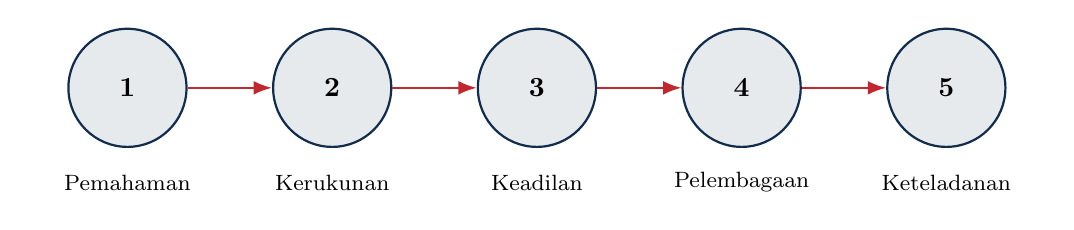
\begin{tikzpicture}[font=\footnotesize]
        \foreach \i/\txt in {1/Pemahaman,2/Kerukunan,3/Keadilan,4/Pelembagaan,5/Keteladanan}
        {
            \pgfmathsetmacro{\x}{(\i-1)*2.6}
            \node[circle, draw=birutuaps, thick, fill=birutuaps!10, minimum size=1.5cm,
                  font=\bfseries] (n\i) at (\x,0) {\i};
            \node[align=center, text width=2.3cm, font=\footnotesize] at (\x,-1.2) {\txt};
        }
        \foreach \i [remember=\i as \last (initially 1)] in {2,...,5}
            \draw[-{Latex}, thick, merahps] (n\last) -- (n\i);
    \end{tikzpicture}}
    \end{center}
    \vspace{3mm}
    \small Kelima jalur ini menjadi peta jalan agar nilai Pancasila tidak berhenti sebagai wacana,
    melainkan benar-benar hidup dalam kelembagaan dan keteladanan bangsa.
\end{frame}

% ---------------------------------------------------------
\begin{frame}{Pengamalan Pancasila dalam Kehidupan Sehari-hari}
    \begin{columns}[T]
        \begin{column}{0.42\textwidth}
            \centering
            \resizebox{\linewidth}{!}{%
            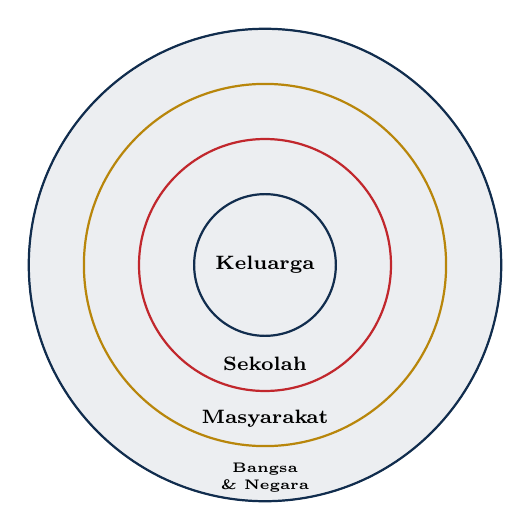
\begin{tikzpicture}[font=\tiny]
                \draw[fill=birutuaps!8] (0,0) circle (3.0);
                \draw[draw=birutuaps, thick] (0,0) circle (0.9);
                \draw[draw=merahps, thick] (0,0) circle (1.6);
                \draw[draw=emasps, thick] (0,0) circle (2.3);
                \draw[draw=birutuaps, thick] (0,0) circle (3.0);
                \node[font=\bfseries\scriptsize] at (0,0) {Keluarga};
                \node[font=\bfseries\scriptsize] at (0,-1.25) {Sekolah};
                \node[font=\bfseries\scriptsize] at (0,-1.95) {Masyarakat};
                \node[font=\bfseries\tiny, align=center, text width=1.6cm] at (0,-2.7) {Bangsa \& Negara};
            \end{tikzpicture}}
        \end{column}
        \begin{column}{0.58\textwidth}
            \small
            \begin{itemize}
                \item \textbf{Keluarga:} Menghormati keluarga, menyelesaikan masalah dengan
                diskusi, saling membantu.
                \item \textbf{Sekolah:} Mematuhi tata tertib, toleransi antarsiswa, mencegah
                perundungan (\textit{bullying}).
                \item \textbf{Masyarakat:} Rukun dengan tetangga, mengutamakan musyawarah,
                tolong-menolong.
                \item \textbf{Bangsa \& Negara:} Toleransi keberagaman, mematuhi hukum, dan
                menyampaikan aspirasi secara bertanggung jawab.
            \end{itemize}
        \end{column}
    \end{columns}
\end{frame}

% =========================================================
\section{Sejarah Penyusunan dan Pengesahan UUD NRI Tahun 1945}

\begin{frame}{Sejarah Penyusunan oleh BPUPK}{A. Sejarah Penyusunan oleh BPUPK}
    \begin{itemize}
        \item UUD Negara Indonesia merdeka dirancang sejak \textbf{29 Mei} hingga
        \textbf{16 Juli 1945} oleh Badan Penyelidik Usaha-Usaha Persiapan Kemerdekaan (BPUPK).
        \item Tiga masalah pokok rancangan UUD yang disampaikan Sukarno: pernyataan Indonesia
        merdeka, Pembukaan UUD, dan Batang Tubuh UUD.
        \item Dibentuk tiga panitia:
        \begin{itemize}
            \item Panitia Perancang Hukum Dasar -- diketuai \textbf{Ir. Sukarno}.
            \item Panitia Perancang Keuangan dan Ekonomi -- diketuai \textbf{Drs. Mohammad Hatta}.
            \item Panitia Perancang Pembelaan Tanah Air -- diketuai \textbf{Abikoesno Tjokrosoejoso}.
        \end{itemize}
        \item Panitia Perancang UUD membentuk \textbf{Panitia Kecil} (diketuai Prof.\ Dr.\ Mr.\ R.\
        Supomo, 11 Juli 1945) dan \textbf{Panitia Penghalus Bahasa} (Husein Djajadiningrat, Agoes
        Salim, Supomo).
    \end{itemize}
\end{frame}

% ---------------------------------------------------------
\begin{frame}{Garis Waktu: Dari BPUPK menuju PPKI}
    \begin{center}
    \resizebox{\linewidth}{!}{%
    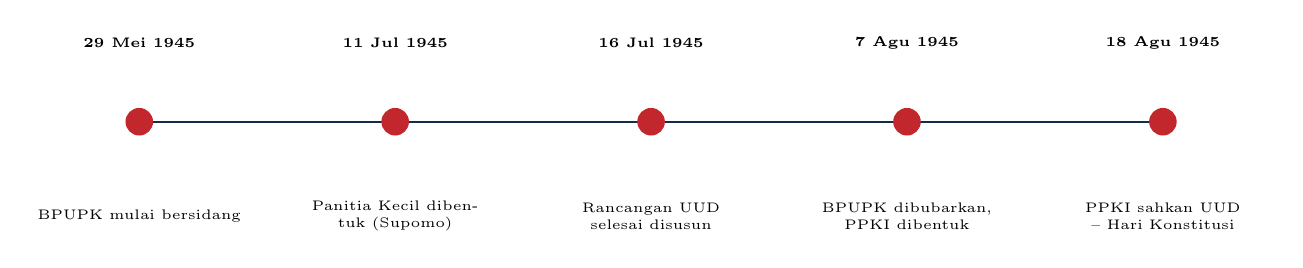
\begin{tikzpicture}[font=\footnotesize]
        \draw[thick, birutuaps] (0,0) -- (13,0);
        \foreach \x/\date/\desc in {
            0/{29 Mei 1945}/{BPUPK mulai bersidang},
            3.25/{11 Jul 1945}/{Panitia Kecil dibentuk (Supomo)},
            6.5/{16 Jul 1945}/{Rancangan UUD selesai disusun},
            9.75/{7 Agu 1945}/{BPUPK dibubarkan, PPKI dibentuk},
            13/{18 Agu 1945}/{PPKI sahkan UUD -- Hari Konstitusi}}
        {
            \node[circle, fill=merahps, minimum size=0.35cm] at (\x,0) {};
            \node[font=\bfseries\tiny, align=center, text width=2.5cm] at (\x,1.0) {\date};
            \node[font=\tiny, align=center, text width=2.6cm] at (\x,-1.2) {\desc};
        }
    \end{tikzpicture}}
    \end{center}
\end{frame}

% ---------------------------------------------------------
\begin{frame}{Pengesahan oleh PPKI dan Peran Tokoh Pemersatu}{B. Pengesahan oleh PPKI dan Peran Tokoh Pemersatu}
    \begin{itemize}
        \item BPUPK dibubarkan pada \textbf{7 Agustus 1945}, digantikan oleh Panitia Persiapan
        Kemerdekaan Indonesia (PPKI).
        \item Sidang pertama, \textbf{18 Agustus 1945} (diperingati sebagai \textbf{Hari
        Konstitusi}), PPKI menetapkan: mengesahkan UUD NRI 1945, memilih \textbf{Ir. Sukarno}
        sebagai Presiden dan \textbf{Drs. Mohammad Hatta} sebagai Wakil Presiden, serta membentuk
        Komite Nasional.
    \end{itemize}
    \vspace{2mm}
    \begin{block}{Peran Mr. Kasman Singodimedjo}
        \small Dipercaya Sukarno dan Hatta untuk meluluhkan hati perwakilan umat Islam (seperti
        Ki Bagoes Hadikoesoemo) agar menyetujui penghapusan tujuh kata dalam Piagam Jakarta
        menjadi \textit{``Ketuhanan Yang Maha Esa''}, demi menjaga keutuhan NKRI. Atas
        pengabdiannya, beliau diangkat sebagai \textbf{Pahlawan Nasional pada tahun 2018}.
    \end{block}
\end{frame}

% =========================================================
\section{Pembukaan UUD NRI Tahun 1945}

\begin{frame}{Kedudukan Pembukaan sebagai Staatsfundamentalnorm}{A. Kedudukan sebagai Staatsfundamentalnorm}
    Pembukaan UUD NRI Tahun 1945 berkedudukan sebagai pokok kaidah negara yang fundamental
    (\textit{staatsfundamentalnorm}), berdasarkan dua unsur utama:
    \vspace{2mm}
    \begin{columns}[T]
        \begin{column}{0.5\textwidth}
            \begin{block}{\small Unsur Terjadinya}
                \footnotesize Disusun dan ditetapkan oleh pembentuk negara (PPKI sebagai wakil
                resmi bangsa Indonesia).
            \end{block}
        \end{column}
        \begin{column}{0.5\textwidth}
            \begin{block}{\small Unsur Isinya}
                \footnotesize Memuat dasar tujuan negara, ketentuan diadakannya UUD, bentuk
                negara, serta dasar falsafah negara (Pancasila).
            \end{block}
        \end{column}
    \end{columns}
    \vspace{3mm}
    \begin{alertblock}{Catatan Yuridis}
        \small Secara yuridis formal, Pembukaan UUD 1945 \textbf{tidak dapat diubah} oleh siapa
        pun. Mengubah Pembukaan sama artinya dengan membubarkan NKRI.
    \end{alertblock}
\end{frame}

% ---------------------------------------------------------
\begin{frame}{Makna Setiap Alinea Pembukaan}{B. Makna Setiap Alinea Pembukaan}
    \begin{center}
    \resizebox{0.98\linewidth}{!}{%
    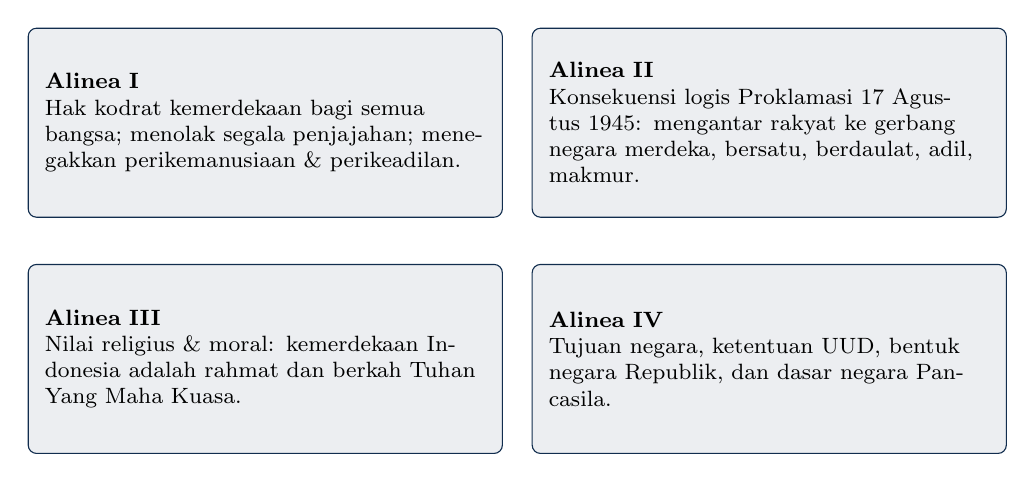
\begin{tikzpicture}[font=\footnotesize,
        box/.style={rectangle, rounded corners=3pt, draw=birutuaps, fill=birutuaps!8,
                    text width=5.6cm, minimum height=2.4cm, align=left, inner sep=6pt}
    ]
        \node[box] at (0,2.1)   {\textbf{Alinea I} \\ Hak kodrat kemerdekaan bagi semua bangsa;
            menolak segala penjajahan; menegakkan perikemanusiaan \& perikeadilan.};
        \node[box] at (6.4,2.1) {\textbf{Alinea II} \\ Konsekuensi logis Proklamasi 17 Agustus
            1945: mengantar rakyat ke gerbang negara merdeka, bersatu, berdaulat, adil, makmur.};
        \node[box] at (0,-0.9)  {\textbf{Alinea III} \\ Nilai religius \& moral: kemerdekaan
            Indonesia adalah rahmat dan berkah Tuhan Yang Maha Kuasa.};
        \node[box] at (6.4,-0.9){\textbf{Alinea IV} \\ Tujuan negara, ketentuan UUD, bentuk
            negara Republik, dan dasar negara Pancasila.};
    \end{tikzpicture}}
    \end{center}
\end{frame}

% ---------------------------------------------------------
\begin{frame}{Cita-Cita Negara dan Kedudukan Pembukaan}{C. Cita-Cita Negara \& Hubungannya dengan Proklamasi/Pasal-Pasal}
    \begin{center}
    \resizebox{0.98\linewidth}{!}{%
    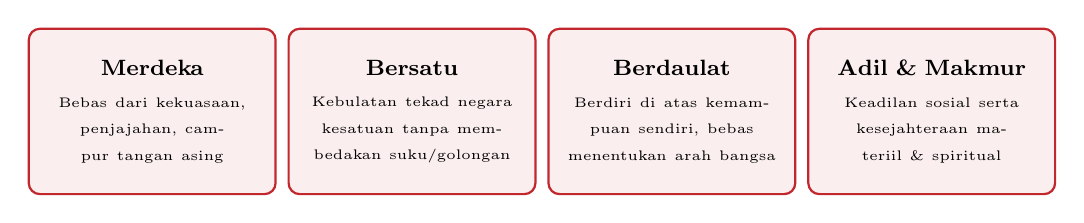
\begin{tikzpicture}[font=\footnotesize,
        box/.style={rectangle, rounded corners=4pt, draw=merahps, thick, fill=merahps!8,
                    text width=2.9cm, minimum height=2.1cm, align=center}
    ]
        \node[box] at (0,0)   {\textbf{Merdeka}\\[2pt]\tiny Bebas dari kekuasaan, penjajahan,
            campur tangan asing};
        \node[box] at (3.3,0) {\textbf{Bersatu}\\[2pt]\tiny Kebulatan tekad negara kesatuan
            tanpa membedakan suku/golongan};
        \node[box] at (6.6,0) {\textbf{Berdaulat}\\[2pt]\tiny Berdiri di atas kemampuan sendiri,
            bebas menentukan arah bangsa};
        \node[box] at (9.9,0) {\textbf{Adil \& Makmur}\\[2pt]\tiny Keadilan sosial serta
            kesejahteraan materiil \& spiritual};
    \end{tikzpicture}}
    \end{center}
    \vspace{4mm}
    \small
    \begin{itemize}
        \item \textbf{Dengan Proklamasi:} Pembukaan adalah perincian dan penegasan lebih lanjut
        dari naskah Proklamasi 17 Agustus 1945.
        \item \textbf{Dengan Pasal-Pasal (Batang Tubuh):} Berhubungan kausal organis --
        Pembukaan menciptakan suasana kebatinan dan cita-cita hukum yang dijabarkan ke dalam
        pasal-pasal UUD NRI 1945.
    \end{itemize}
\end{frame}

% =========================================================
\section{Dinamika Pelaksanaan UUD NRI Tahun 1945}

\begin{frame}{Pengantar Konstitusi}{A. Pengantar Konstitusi}
    \begin{itemize}
        \item Istilah \textbf{konstitusi} berasal dari bahasa Prancis (\textit{constituer}) dan
        Inggris (\textit{constitution}), berarti ``membentuk suatu negara''.
        \item UUD NRI Tahun 1945 berkedudukan sebagai konstitusi tertulis (\textit{documentary
        constitution}) dan merupakan \textbf{sumber hukum tertinggi}.
        \item Segala peraturan perundang-undangan di Indonesia harus bersumber pada Pancasila
        dan UUD 1945.
    \end{itemize}
\end{frame}

% ---------------------------------------------------------
\begin{frame}{Pembabakan Dinamika Pelaksanaan UUD}{B. Pembabakan Dinamika Pelaksanaan UUD}
    \begin{center}
    \resizebox{\linewidth}{!}{%
    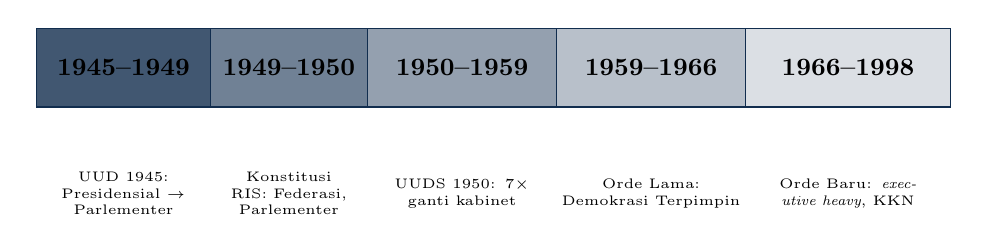
\begin{tikzpicture}[font=\footnotesize]
        \foreach \start/\w/\lbl/\clr in {
            0/2.2/{1945--1949}/birutuaps!80,
            2.2/2.0/{1949--1950}/birutuaps!60,
            4.2/2.4/{1950--1959}/birutuaps!45,
            6.6/2.4/{1959--1966}/birutuaps!30,
            9.0/2.6/{1966--1998}/birutuaps!15}
        {
            \draw[fill=\clr, draw=birutuaps] (\start,0) rectangle ++(\w,1.0);
            \node[font=\bfseries\small] at ({\start+\w/2},0.5) {\lbl};
        }
        \node[font=\tiny, align=center, text width=2.2cm] at (1.1,-1.1)
            {UUD 1945: Presidensial $\to$ Parlementer};
        \node[font=\tiny, align=center, text width=2.0cm] at (3.2,-1.1)
            {Konstitusi RIS: Federasi, Parlementer};
        \node[font=\tiny, align=center, text width=2.4cm] at (5.4,-1.1)
            {UUDS 1950: 7$\times$ ganti kabinet};
        \node[font=\tiny, align=center, text width=2.4cm] at (7.8,-1.1)
            {Orde Lama: Demokrasi Terpimpin};
        \node[font=\tiny, align=center, text width=2.6cm] at (10.3,-1.1)
            {Orde Baru: \textit{executive heavy}, KKN};
    \end{tikzpicture}}
    \end{center}
\end{frame}

% ---------------------------------------------------------
\begin{frame}{Rincian Pembabakan Dinamika Pelaksanaan UUD}
    \small
    \renewcommand{\arraystretch}{1.35}
    \begin{tabularx}{\linewidth}{@{}lX@{}}
        \toprule
        \textbf{Periode} & \textbf{Karakteristik Utama} \\ \midrule
        1945--1949 & Pelaksanaan UUD belum optimal (fokus mempertahankan kemerdekaan);
        perubahan sistem Presidensial $\to$ Parlementer via Maklumat 14 November 1945. \\
        1949--1950 & Bentuk negara berubah menjadi Serikat/Federasi dengan sistem pemerintahan
        Parlementer. \\
        1950--1959 & Kembali ke Negara Kesatuan namun sistem Parlementer menyebabkan
        ketidakstabilan (7 kali pergantian kabinet). \\
        1959--1966 & Kembali ke UUD 1945 (Dekrit Presiden 5 Juli 1959); berlaku Demokrasi
        Terpimpin; muncul penyimpangan seperti Presiden Seumur Hidup. \\
        1966--1998 & Bermaksud melaksanakan Pancasila \& UUD 1945 murni-konsekuen, namun
        terjadi kekuasaan terpusat (\textit{executive heavy}) dan maraknya KKN. \\
        \bottomrule
    \end{tabularx}
\end{frame}

% =========================================================
\section{Amendemen UUD NRI Tahun 1945 (1999--2002)}

\begin{frame}{Lima Kesepakatan Dasar Amendemen}{A. Lima Kesepakatan Dasar Amendemen}
    \begin{center}
    \resizebox{0.98\linewidth}{!}{%
    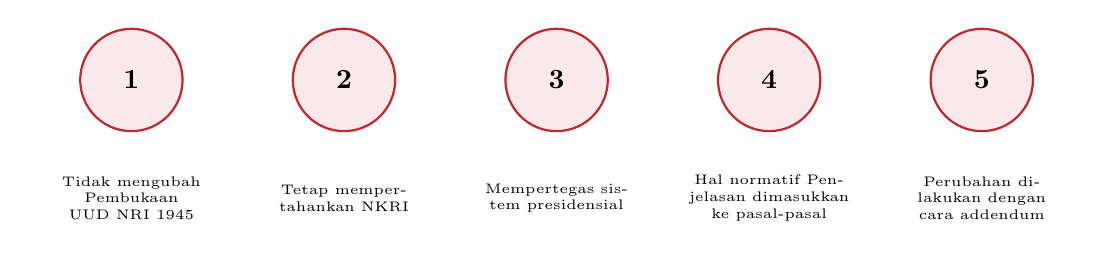
\begin{tikzpicture}[font=\footnotesize]
        \foreach \i/\txt in {
            1/{Tidak mengubah Pembukaan UUD NRI 1945},
            2/{Tetap mempertahankan NKRI},
            3/{Mempertegas sistem presidensial},
            4/{Hal normatif Penjelasan dimasukkan ke pasal-pasal},
            5/{Perubahan dilakukan dengan cara addendum}}
        {
            \pgfmathsetmacro{\x}{(\i-1)*2.7}
            \node[circle, draw=merahps, thick, fill=merahps!10, minimum size=1.3cm,
                  font=\bfseries] (n\i) at (\x,0) {\i};
            \node[align=center, text width=2.4cm, font=\tiny] at (\x,-1.5) {\txt};
        }
    \end{tikzpicture}}
    \end{center}
\end{frame}

% ---------------------------------------------------------
\begin{frame}{Perubahan Struktural: Sebelum vs Setelah Amendemen}{B. Perubahan Struktural Utama}
    \begin{center}
    \resizebox{0.86\linewidth}{!}{%
    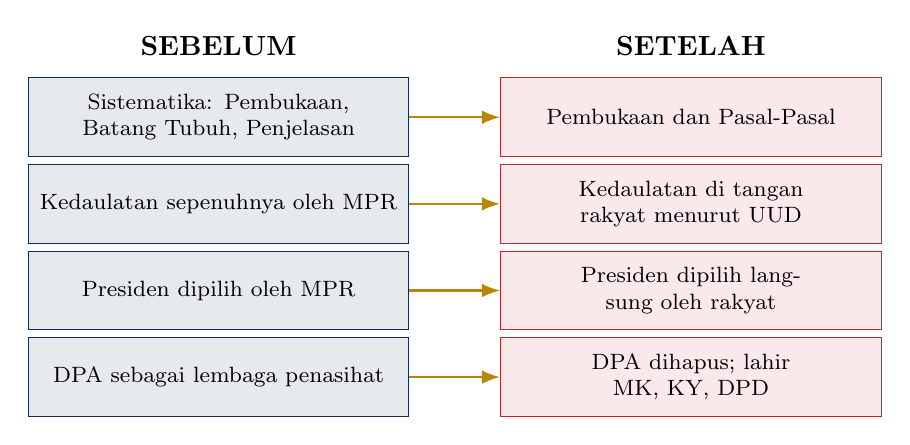
\begin{tikzpicture}[font=\footnotesize,
        boxL/.style={rectangle, draw=birutuaps, fill=birutuaps!10, text width=4.6cm,
                     minimum height=1.0cm, align=center},
        boxR/.style={rectangle, draw=merahps, fill=merahps!10, text width=4.6cm,
                     minimum height=1.0cm, align=center}
    ]
        \node[font=\bfseries] at (-3.0,2.55) {SEBELUM};
        \node[font=\bfseries] at (3.0,2.55)  {SETELAH};
        \foreach \y/\l/\r in {
            1.65/{Sistematika: Pembukaan, Batang Tubuh, Penjelasan}/{Pembukaan dan Pasal-Pasal},
            0.55/{Kedaulatan sepenuhnya oleh MPR}/{Kedaulatan di tangan rakyat menurut UUD},
            -0.55/{Presiden dipilih oleh MPR}/{Presiden dipilih langsung oleh rakyat},
            -1.65/{DPA sebagai lembaga penasihat}/{DPA dihapus; lahir MK, KY, DPD}}
        {
            \node[boxL] (L) at (-3.0,\y) {\l};
            \node[boxR] (R) at (3.0,\y)  {\r};
            \draw[-{Latex}, thick, emasps] (L) -- (R);
        }
    \end{tikzpicture}}
    \end{center}
\end{frame}

% ---------------------------------------------------------
\begin{frame}{Peran dan Kewenangan Mahkamah Konstitusi (MK)}{C. Peran dan Kewenangan MK}
    \begin{center}
    \resizebox{0.8\linewidth}{!}{%
    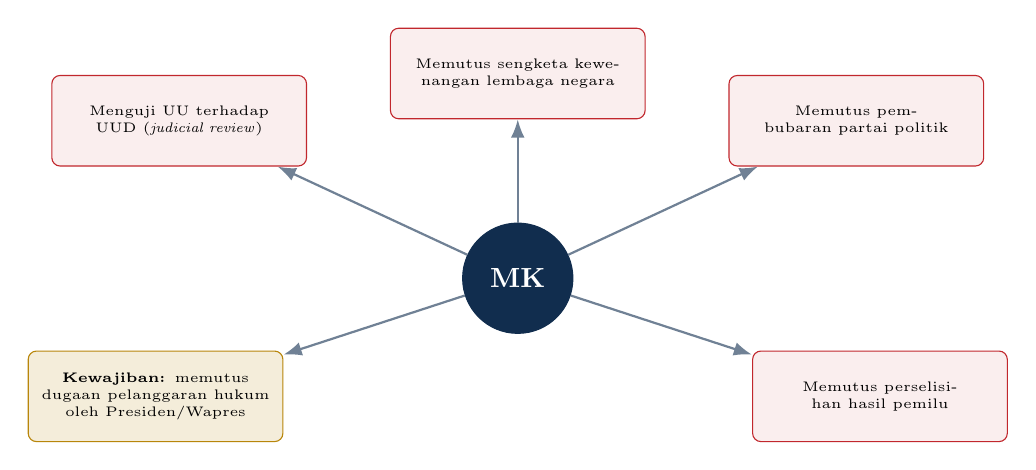
\begin{tikzpicture}[font=\footnotesize,
        center/.style={circle, draw=birutuaps, fill=birutuaps, text=white, font=\bfseries,
                       minimum size=1.4cm},
        leaf/.style={rectangle, rounded corners=3pt, draw=merahps, fill=merahps!8,
                     text width=3.0cm, minimum height=1.15cm, align=center, font=\tiny}
    ]
        \node[center] (mk) at (0,0) {MK};
        \node[leaf] (k1) at (-4.3,2.0) {Menguji UU terhadap UUD (\textit{judicial review})};
        \node[leaf] (k2) at (0,2.6)    {Memutus sengketa kewenangan lembaga negara};
        \node[leaf] (k3) at (4.3,2.0)  {Memutus pembubaran partai politik};
        \node[leaf] (k4) at (4.6,-1.5) {Memutus perselisihan hasil pemilu};
        \node[leaf, draw=emasps, fill=emasps!15] (kw) at (-4.6,-1.5)
            {\textbf{Kewajiban:} memutus dugaan pelanggaran hukum oleh Presiden/Wapres};
        \foreach \n in {k1,k2,k3,k4,kw}
            \draw[-{Latex}, thick, birutuaps!60] (mk) -- (\n);
    \end{tikzpicture}}
    \end{center}
    \vspace{1mm}
    {\scriptsize\centering \textbf{Peran Strategis:} \textit{Guardian of the Constitution}, \textit{Final
    Interpreter of the Constitution}, \textit{Guardian of Democracy}, \textit{Protector of Human
    Rights}.\par}
\end{frame}

% =========================================================
\section{Hak dan Kewajiban Warga Negara dalam UUD NRI Tahun 1945}

\begin{frame}{Konsep Dasar dan Prinsip Hak \& Kewajiban}{A. Konsep Dasar \& Prinsip}
    \begin{columns}[T]
        \begin{column}{0.55\textwidth}
            \small
            \begin{itemize}
                \item \textbf{Hak Konstitusional:} Hak yang dijamin dalam UUD NRI Tahun 1945.
                \item \textbf{Kewajiban:} Sesuatu yang harus dilaksanakan dengan penuh tanggung
                jawab.
                \item \textbf{Prinsip Hubungan (Kausalitas):} Bersifat timbal balik
                (\textit{reciprocity}) dan tidak dapat dipisahkan; pelaksanaannya harus seimbang.
            \end{itemize}
        \end{column}
        \begin{column}{0.45\textwidth}
            \centering
            \resizebox{\linewidth}{!}{%
            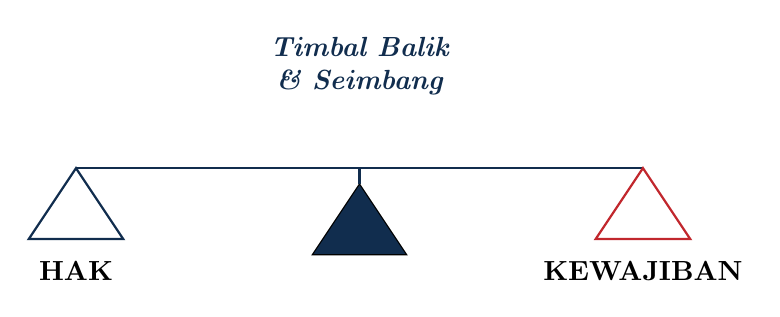
\begin{tikzpicture}[font=\small]
                \draw[fill=birutuaps] (0,-1.2) -- (-0.6,-2.1) -- (0.6,-2.1) -- cycle;
                \draw[thick, birutuaps] (-3.6,-1.0) -- (3.6,-1.0);
                \draw[thick, birutuaps] (0,-1.0) -- (0,-1.2);
                \draw[thick, birutuaps] (-3.6,-1.0) -- (-4.2,-1.9) -- (-3.0,-1.9) -- cycle;
                \draw[thick, merahps]   (3.6,-1.0)  -- (3.0,-1.9)  -- (4.2,-1.9)  -- cycle;
                \node[font=\bfseries] at (-3.6,-2.3) {HAK};
                \node[font=\bfseries] at (3.6,-2.3)  {KEWAJIBAN};
                \node[font=\bfseries\itshape, birutuaps, align=center, text width=4.5cm]
                    at (0,0.3) {Timbal Balik \\ \& Seimbang};
            \end{tikzpicture}}
        \end{column}
    \end{columns}
\end{frame}

% ---------------------------------------------------------
\begin{frame}{Rincian Jaminan Hak dan Kewajiban Berdasarkan Pasal}{B. Rincian Berdasarkan Pasal}
    \footnotesize
    \renewcommand{\arraystretch}{1.12}
    \begin{tabularx}{\linewidth}{@{}lX@{}}
        \toprule
        \textbf{Pasal} & \textbf{Isi Singkat} \\ \midrule
        27 & Kedudukan sama dalam hukum/pemerintahan (Ayat 1); hak pekerjaan dan penghidupan
        layak (Ayat 2); hak dan kewajiban bela negara (Ayat 3). \\
        28A--28C & Hak hidup, berkeluarga, perlindungan anak, mengembangkan diri lewat
        pendidikan dan IPTEK. \\
        28D--28F & Kepastian hukum yang adil, hak bekerja, kesempatan sama dalam pemerintahan,
        kebebasan beragama, hak berkomunikasi. \\
        28G--28H & Perlindungan diri, bebas dari penyiksaan, hak lingkungan hidup sehat dan
        jaminan sosial. \\
        28I & Hak yang tidak dapat dikurangi dalam keadaan apa pun (\textit{non-derogable
        rights}) dan perlindungan dari diskriminasi. \\
        28J & Kewajiban menghormati HAM orang lain dan tunduk pada pembatasan UU. \\
        29 & Negara berdasar Ketuhanan Yang Maha Esa; jaminan kemerdekaan memeluk agama. \\
        30 & Hak dan kewajiban warga negara dalam usaha pertahanan dan keamanan negara. \\
        31 \& 32 & Hak pendidikan (wajib belajar dasar, anggaran minimal 20\%) dan pemajuan
        kebudayaan nasional/bahasa daerah. \\
        33 \& 34 & Perekonomian atas asas kekeluargaan; fakir miskin dan anak terlantar
        dipelihara negara. \\
        \bottomrule
    \end{tabularx}
\end{frame}

% ---------------------------------------------------------
\begin{frame}{Contoh Penerapan Hak dan Kewajiban Sehari-hari}{C. Contoh Penerapan Sehari-hari}
    \begin{columns}[T]
        \begin{column}{0.5\textwidth}
            \begin{block}{\centering Contoh Hak}
                \small
                \begin{itemize}
                    \item Memeluk agama sesuai keyakinan.
                    \item Menyuarakan pendapat.
                    \item Mendapat pendidikan.
                    \item Memiliki properti secara legal.
                    \item Diperlakukan sama di mata hukum.
                \end{itemize}
            \end{block}
        \end{column}
        \begin{column}{0.5\textwidth}
            \begin{block}{\centering Contoh Kewajiban}
                \small
                \begin{itemize}
                    \item Membayar pajak.
                    \item Menaati aturan hukum.
                    \item Menghormati hak orang lain.
                    \item Menjaga sarana umum.
                    \item Menjaga kebersihan lingkungan.
                \end{itemize}
            \end{block}
        \end{column}
    \end{columns}
\end{frame}

% =========================================================
\section{Referensi}
\begin{frame}[allowframebreaks]{Sumber Referensi}
    \begin{thebibliography}{9}
        \setbeamertemplate{bibliography item}[book] % Icon buku

        \bibitem{bumiaksara}
        Tim Penulis.
        \newblock \textit{Pendidikan Pancasila untuk SMK/MAK Kelas XI (Kurikulum Merdeka)}.
        \newblock Jakarta: PT Bumi Aksara.

        \bibitem{mpr}
        Sekretariat Jenderal MPR RI.
        \newblock \textit{Undang-Undang Dasar Negara Republik Indonesia Tahun 1945}.

    \end{thebibliography}
\end{frame}

% =========================================================
\begin{frame}
    \centering
    \Huge \textbf{Terima Kasih} \\
    \vspace{0.7cm}
    \large Mari Berdiskusi! \\
    \vspace{0.3cm}
    \normalsize Apakah ada pertanyaan?
\end{frame}

\end{document}
